%\documentclass[tikz, border=5pt]{standalone}
\begin{document}
	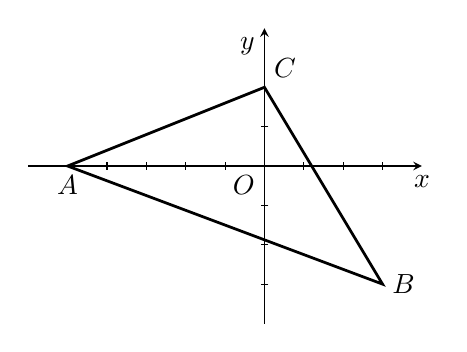
\begin{tikzpicture}[>=stealth, scale=0.5]
		% 绘制坐标轴
		\draw[->] (-6,0) -- (4,0) node[below] {$x$}; % x轴(带箭头和标签)
		\draw[->] (0,-4) -- (0,3.5) node[below left] {$y$}; % y轴(带箭头和标签)
		\node at (0,0) [below left] {$O$};           % 原点O的标签

		% 绘制所有小刻度线(从 -1 到 2,每隔 1 单位画竖线)
		\foreach \x in {-4, -3,...,3} {
			\draw (\x, 0.1) -- (\x, -0.1);  % 小竖线(长 0.2 单位)
		}
		\foreach \y in {-3,-2,...,1} {
			\draw (0.1,\y) -- (-0.1,\y);  % 小竖线(长 0.2 单位)
		}
		
		% 定义各关键点坐标(可根据图形比例调整)
		\coordinate (A) at (-5,0);   % 点 $A$
		\coordinate (B)  at (3,-3);    % 点 $B$
		\coordinate (C) at (0,2);    % 点 $C$
		
		% 绘制连线
		\draw [line width=1pt] (A) -- (B) -- (C) -- cycle; % 绘制三角形
		
		% 标记各点的标签 实心圆点
%		\fill (G) circle (2pt) node [right] {$G$};  % 带标签的实心点
		\node at (A) [below] {$A$}; 
		\node at (B) [right] {$B$}; 
		\node at (C) [above right] {$C$}; 
		
	\end{tikzpicture}
\end{document}
